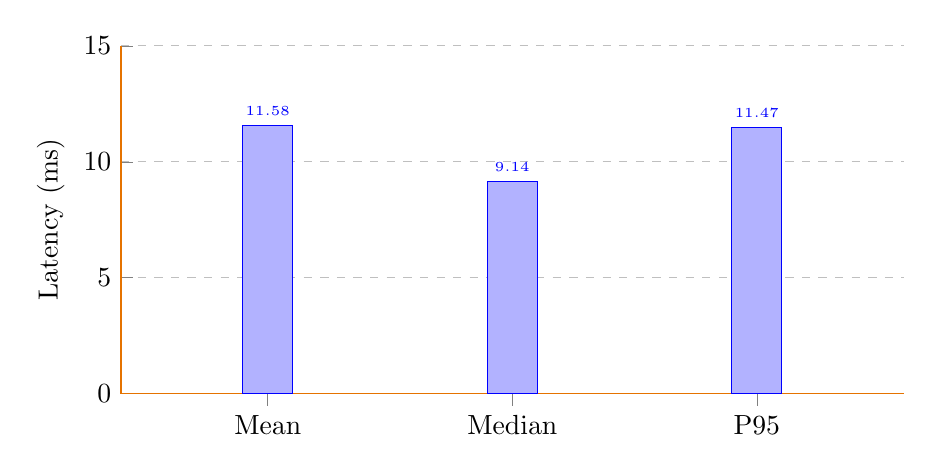
\begin{tikzpicture}
\begin{axis}[
    ybar,
    enlarge x limits=0.3,
    ylabel={Latency (ms)},
    symbolic x coords={Mean, Median, P95},
    xtick=data,
    nodes near coords,
    nodes near coords align={vertical},
    every node near coord/.append style={font=\tiny\bfseries},
    ymin=0, ymax=15,
    width=0.95\textwidth,
    height=6cm,
    bar width=18pt,
    fill=orange!80!black,
    draw=orange!90!black,
    ymajorgrids=true,
    grid style=dashed,
    axis lines*=left,
]
\addplot coordinates {(Mean,11.58) (Median,9.14) (P95,11.47)};
\end{axis}
\end{tikzpicture}
